\documentclass[11pt]{article}

\usepackage[margin=1in]{geometry}
\usepackage[T1]{fontenc}
\usepackage[utf8]{inputenc}
\usepackage{lmodern}
\usepackage{microtype}
\usepackage{booktabs}
\usepackage{longtable}
\usepackage{array}
\usepackage{enumitem}
\usepackage{hyperref}
\usepackage{xcolor}
\usepackage{tikz}
\usetikzlibrary{arrows.meta, positioning, fit}

\hypersetup{
  colorlinks=true,
  linkcolor=blue,
  urlcolor=blue,
  citecolor=blue
}

\setlist[itemize]{leftmargin=1.2em}
\setlist[enumerate]{leftmargin=1.4em}
\renewcommand{\arraystretch}{1.15}

\newcommand{\Product}{TenaOS}
\newcommand{\Gemma}{Gemma 4 E4B}
\newcommand{\OpenMRS}{OpenMRS}
\newcommand{\CIEL}{CIEL}
\newcommand{\WHO}{WHO/MSF}

\title{\Product: A Local-First Clinical AI Operating System for Standards-Based Primary Care}
\author{TenaOS Project}
\date{Gemma 4 Good Technical Report}

\begin{document}
\maketitle

\begin{abstract}
\Product{} is a local-first clinical AI operating system that lets primary-care clinics build and operate standards-based digital health workflows through natural language. It combines \OpenMRS{}, \Gemma{}, a \WHO{} guideline knowledge base, a \CIEL{} terminology knowledge base, deterministic middleware, and clinician review inside a locally deployable stack.

The problem \Product{} addresses is implementation failure. Clinics need forms, terminology mappings, reporting logic, guideline support, and localized patient communication, but the expertise to configure those systems is usually external, expensive, and temporary. \Product{} turns that implementation work into a local, auditable, clinician-reviewed agent workflow.

The system runs as a single local container with \OpenMRS{}, MariaDB, Qdrant, \Gemma{} served through \texttt{llama.cpp}, and the TenaAgent orchestration service. TenaAgent implements form building, scribing, evidence-grounded clinical decision support, patient education, reporting, and lab lookup. The model never writes directly to \OpenMRS{}. It operates through allow-listed tools and structured draft stores; final writes go through deterministic validation and clinician approval.

Measured implementation artifacts include a local \CIEL{} SQLite store with 58,687 concepts and 298,905 mappings, a \WHO{} guideline index with 69,476 chunks, Qdrant snapshots for both guideline and \CIEL{} retrieval, and a LoRA/SFT corpus with 16,005 validated task-tagged traces split into 18,909 training, 1,071 validation, and 1,109 held-out test conversations. Internal technical form-builder evaluation completed 147/147 prompts with 0 failures, 0.465 mean concept-cluster recall, 0.993 schema-valid rate, and 17.97 s median latency.
\end{abstract}

\section{Status, Naming, and Model Scope}

This report uses \Product{} as the canonical product name. The technical artifacts, code paths, and diagrams in this report use \Product{} consistently.

All runtime code, artifacts, and evaluation results in this report refer to \Gemma{} BF16 GGUF served via \texttt{llama.cpp}, with the Gemma multimodal projector for audio input.

\section{Contributions}

\Product{} makes four technical contributions.

\begin{enumerate}
  \item \textbf{A local-first clinical AI runtime.} \Product{} packages \OpenMRS{}, \Gemma{}, local guideline retrieval, local terminology retrieval, and TenaAgent into a single deployable stack.
  \item \textbf{Two complementary local knowledge bases.} The \WHO{} knowledge base grounds recommendations and patient materials in guideline evidence; the \CIEL{} knowledge base resolves natural language to standards-based \OpenMRS{} concepts.
  \item \textbf{A constrained clinical agent pattern.} \Gemma{} interacts through allow-listed tools, retrieval services, draft stores, deterministic validators, and \OpenMRS{} writers instead of uncontrolled free-text actions. The architecture treats the model as a planner and proposer, while concept validation, schema construction, query compilation, and persistence stay deterministic.
  \item \textbf{A GEPA-first adaptation path.} The central adaptation claim is that many clinical agent failures are instruction and tool-use failures before they are weight failures. \Product{} therefore optimizes prompts against the real production pipeline with GEPA before training LoRA adapters on validated traces.
\end{enumerate}

\section{Design Requirements}

\Product{} targets clinics that cannot assume continuous internet, cloud inference, or a local implementation team. The system is built around six requirements:

\begin{itemize}
  \item \textbf{Local ownership:} patient data and model inference stay on facility-owned infrastructure.
  \item \textbf{Standards compatibility:} \OpenMRS{} remains the record system; \CIEL{} and FHIR-style query plans preserve interoperability.
  \item \textbf{Clinical review:} every AI-generated clinical artifact remains reviewable and editable by a clinician.
  \item \textbf{Deterministic trust boundary:} middleware validates concept IDs, datatypes, retired status, schema structure, reporting plans, and \OpenMRS{} writes.
  \item \textbf{Evidence grounding:} CDS and patient education search local \WHO{} evidence rather than answering from model memory.
  \item \textbf{Auditability:} tool calls, retrieval steps, drafts, and final outputs are persisted or streamed as traces.
\end{itemize}

\section{Runtime Architecture}

At a high level, \Product{} converts natural clinical language into standards-based clinical artifacts.

\begin{figure}[h]
\centering
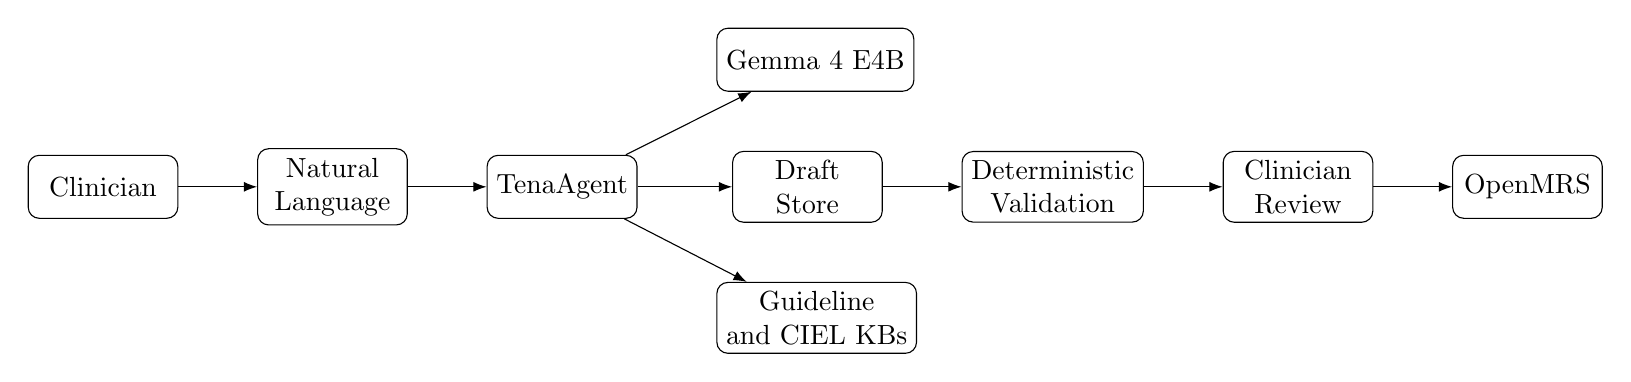
\begin{tikzpicture}[
  box/.style={draw, rounded corners, align=center, minimum height=0.8cm, minimum width=1.9cm},
  arrow/.style={-Latex}
]
\node[box] (clinician) {Clinician};
\node[box, right=of clinician] (input) {Natural\\Language};
\node[box, right=of input] (agent) {TenaAgent};
\node[box, above right=0.8cm and 1.0cm of agent] (gemma) {\Gemma};
\node[box, right=1.2cm of agent] (draft) {Draft\\Store};
\node[box, below right=0.8cm and 1.0cm of agent] (kb) {Guideline\\and CIEL KBs};
\node[box, right=of draft] (validate) {Deterministic\\Validation};
\node[box, right=of validate] (review) {Clinician\\Review};
\node[box, right=of review] (openmrs) {\OpenMRS};

\draw[arrow] (clinician) -- (input);
\draw[arrow] (input) -- (agent);
\draw[arrow] (agent) -- (gemma);
\draw[arrow] (agent) -- (kb);
\draw[arrow] (agent) -- (draft);
\draw[arrow] (draft) -- (validate);
\draw[arrow] (validate) -- (review);
\draw[arrow] (review) -- (openmrs);
\end{tikzpicture}
\caption{The TenaOS safety invariant: model proposals pass through tools, draft stores, deterministic validation, and clinician review before persistence.}
\end{figure}

The deployed runtime is a single-container stack. nginx is the only public ingress. TenaAgent, \OpenMRS{}, Qdrant, Gemma, and both knowledge-base daemons communicate on container-local ports.

\begin{figure}[h]
\centering
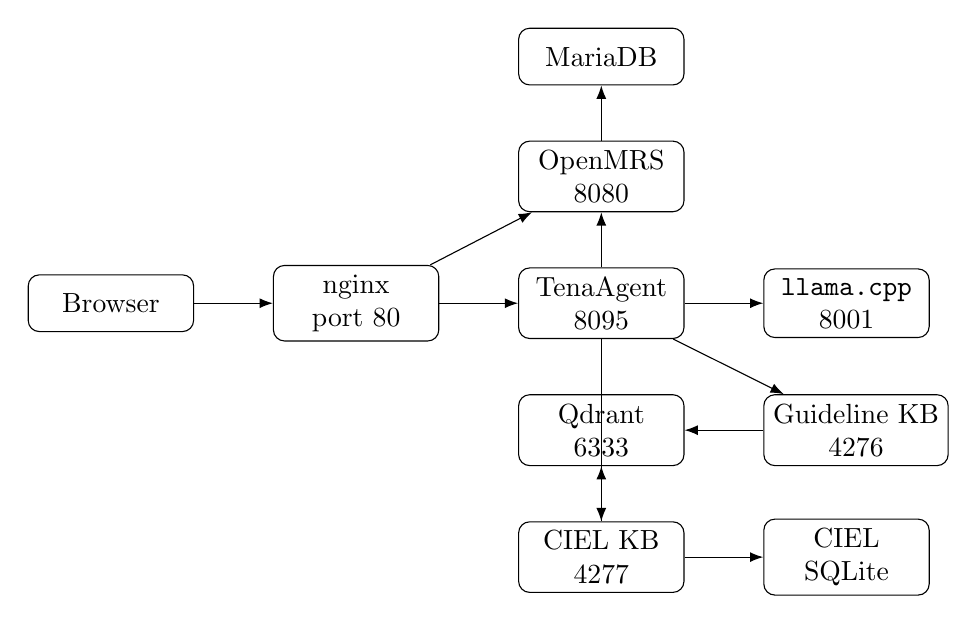
\begin{tikzpicture}[
  box/.style={draw, rounded corners, align=center, minimum height=0.72cm, minimum width=2.1cm},
  arrow/.style={-Latex},
  node distance=0.7cm and 1.0cm
]
\node[box] (browser) {Browser};
\node[box, right=of browser] (nginx) {nginx\\port 80};
\node[box, right=of nginx] (agent) {TenaAgent\\8095};
\node[box, above=of agent] (openmrs) {\OpenMRS\\8080};
\node[box, above=of openmrs] (mariadb) {MariaDB};
\node[box, right=of agent] (llama) {\texttt{llama.cpp}\\8001};
\node[box, below=of agent] (qdrant) {Qdrant\\6333};
\node[box, right=of qdrant] (guideline) {Guideline KB\\4276};
\node[box, below=of qdrant] (ciel) {CIEL KB\\4277};
\node[box, right=of ciel] (sqlite) {CIEL\\SQLite};

\draw[arrow] (browser) -- (nginx);
\draw[arrow] (nginx) -- (agent);
\draw[arrow] (nginx) -- (openmrs);
\draw[arrow] (agent) -- (llama);
\draw[arrow] (agent) -- (guideline);
\draw[arrow] (agent) -- (ciel);
\draw[arrow] (agent) -- (openmrs);
\draw[arrow] (guideline) -- (qdrant);
\draw[arrow] (ciel) -- (qdrant);
\draw[arrow] (ciel) -- (sqlite);
\draw[arrow] (openmrs) -- (mariadb);
\end{tikzpicture}
\caption{Single-container runtime architecture.}
\end{figure}

\section{Local Knowledge Systems}

\Product{} has two local knowledge systems because clinical evidence and clinical terminology serve different roles.

\begin{itemize}
  \item The \WHO{} guideline knowledge base answers: what does the evidence or protocol say?
  \item The \CIEL{} terminology knowledge base answers: which standard concept should represent this clinical idea in \OpenMRS{}?
\end{itemize}

\subsection{WHO/MSF Guideline Knowledge Base}

The \WHO{} knowledge base is composed of WHO and MSF clinical guidance documents, including clinical practice guidelines, pocket guides, technical reports, rapid advice, consolidated guidance, and MSF protocol-style material. The offline build pipeline lives in \texttt{/var/www/TenaOS\_DeepSeek/kb-pipeline}.

The extraction begins with Pulse OCR. The extraction script uploads PDFs to the Pulse \texttt{/extract} API in asynchronous mode and stores normalized JSON for each document. Each result preserves extracted markdown, page count, extraction ID, bounding boxes, warnings, optional footnote references, large-document S3 result handling, resume metadata, and a page-budget tracker. The Pulse extraction script tracks a 19,900-page extraction budget.

The current build tree contains 401 chunk JSONL files and 69,476 guideline chunks. The resulting \texttt{who\_msf\_guidelines.snapshot} is about 448.8 MB.

\begin{figure}[h]
\centering

\begin{tikzpicture}[
  box/.style={draw, rounded corners, align=center, minimum height=0.75cm, minimum width=1.8cm},
  arrow/.style={-Latex},
  node distance=0.8cm and 0.65cm
]
\node[box] (pdf) {PDFs};
\node[box, right=of pdf] (pulse) {Pulse\\OCR};
\node[box, right=of pulse] (docling) {Docling\\JSON};
\node[box, right=of docling] (chunk) {Chunk\\Enrich};
\node[box, right=of chunk] (embed) {EmbedGemma\\BM25};
\node[box, right=of embed] (qdrant) {Qdrant\\Snapshot};
\draw[arrow] (pdf) -- (pulse);
\draw[arrow] (pulse) -- (docling);
\draw[arrow] (docling) -- (chunk);
\draw[arrow] (chunk) -- (embed);
\draw[arrow] (embed) -- (qdrant);
\end{tikzpicture}
\caption{WHO/MSF guideline build pipeline.}
\end{figure}

The build pipeline converts cleaned markdown into Docling JSON, classifies documents, fixes heading levels, chunks documents, enriches metadata, post-processes chunks, and backfills metadata. Shared chunking logic identifies recommendation signals such as ``WHO recommends,'' ``It is recommended that,'' ``Good practice statement,'' and GRADE certainty symbols. It classifies content into recommendation, implementation, evidence-to-decision, methods/PICO, background, research gap, annex, and scope chunks.

Each chunk stores heading paths, provenance, source URL, document type, disease area, content hash, version date, token count, recommendation number, and retrieval priority. Current or actionable chunks receive higher retrieval priority; superseded chunks can be hard-dropped with retrieval priority 0.0.

The embedding stage contextualizes each chunk as heading path plus body text and embeds it with EmbedGemma 300M into 768-dimensional vectors. Long chunks are split into up to three 10,000-character windows, embedded independently, mean-pooled, and normalized. The Qdrant build aligns chunk IDs with embeddings, cleans OCR artifacts, filters low-quality snippets, computes BM25 sparse vectors, and stores dense vector \texttt{embedgemma} plus sparse vector \texttt{bm25}.

At runtime, the KB daemon exposes local \texttt{/health}, \texttt{/stats}, and \texttt{/search} endpoints. Retrieval supports lexical BM25, semantic EmbedGemma, and reciprocal-rank fusion. The reranker performs corruption filtering, synonym expansion, action-query detection, content-type boosts, actionability boosts for dose/route/frequency text, domain coherence penalties, source diversity penalties, condition/title exclusions, population/intent reranking, and low-confidence flags.

\subsection{CIEL Terminology Knowledge Base}

\CIEL{} is the terminology layer that makes \Product{} interoperable with \OpenMRS{}. The local SQLite store is built from an OpenConceptLab CIEL export. The checked local artifact is CIEL \texttt{v2026-03-23}.

The measured SQLite artifact contains 58,687 concepts, 3,205 retired concepts, 298,905 mappings, 8,545 Q-and-A edges, 3,259 concept-set edges, and 58,687 concept bundles with search text.

\begin{figure}[h]
\centering
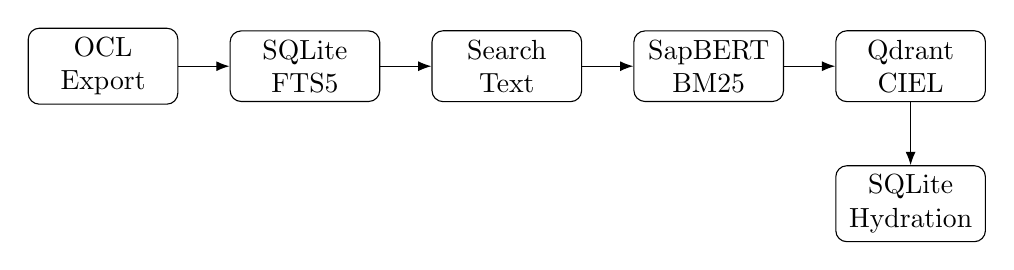
\begin{tikzpicture}[
  box/.style={draw, rounded corners, align=center, minimum height=0.75cm, minimum width=1.9cm},
  arrow/.style={-Latex},
  node distance=0.8cm and 0.65cm
]
\node[box] (ocl) {OCL\\Export};
\node[box, right=of ocl] (sqlite) {SQLite\\FTS5};
\node[box, right=of sqlite] (text) {Search\\Text};
\node[box, right=of text] (vectors) {SapBERT\\BM25};
\node[box, right=of vectors] (qdrant) {Qdrant\\CIEL};
\node[box, below=of qdrant] (hydrate) {SQLite\\Hydration};
\draw[arrow] (ocl) -- (sqlite);
\draw[arrow] (sqlite) -- (text);
\draw[arrow] (text) -- (vectors);
\draw[arrow] (vectors) -- (qdrant);
\draw[arrow] (qdrant) -- (hydrate);
\end{tikzpicture}
\caption{CIEL terminology build and runtime hydration.}
\end{figure}

The SQLite build streams the OCL export and writes source metadata, concept bundles, concept mappings, and an FTS5 index. Each concept bundle preserves raw concept JSON and stores UUID, display name, class, datatype, retired status, locales, names, descriptions, answers, set members, external mappings, incoming relationships, source version, and generated search text.

Search text is built from preferred names, synonyms, descriptions, answer labels, set-member labels, external source codes, and relationship labels. SQLite remains the authority for deterministic lookups and bundle expansion. It supports exact search, FTS5 fallback, Q-and-A answer expansion, concept-set member expansion, and form-ready seed discovery.

The semantic CIEL index uses SapBERT for dense concept embeddings and a shared BM25 encoder for sparse vectors. The Qdrant collection \texttt{ciel\_concepts} stores dense vector \texttt{sapbert}, sparse vector \texttt{bm25}, and payload fields for concept ID, UUID, display name, class, datatype, retired status, locales, set status, external mapping sources, and source version. The local \texttt{ciel\_concepts.snapshot} is about 326.3 MB.

Runtime CIEL discovery is hybrid. Qdrant returns candidate concept IDs, then SQLite hydrates them into authoritative concept bundles. The runtime never trusts vector search alone. Final decisions use class, datatype, retired status, duplicate concept checks, answer availability, set membership, and \OpenMRS{} UUID compatibility.

\section{Feature Architecture}

\subsection{Natural-Language Form Builder}

The form builder is the most mature workflow and the primary GEPA optimization target. The production pipeline reviews the request against the \WHO{} KB, produces a structured question worklist, resolves worklist items against \CIEL{}, commits fields into a draft basket, runs a bounded coverage-repair pass, builds an \OpenMRS{} schema, produces a deterministic summary, and publishes only after approval.

\OpenMRS{} form publication is a three-step REST operation: create Form metadata, upload the JSON schema as ClobData, and bind the schema as a form resource. If a later step fails, the created form is retired so only usable forms appear in the form list.

\subsection{SOAP Scribe}

The scribe accepts text or voice. For voice input, the route accepts multipart audio, converts it to 16 kHz mono WAV with \texttt{ffmpeg}, base64-encodes it, and sends it to Gemma using an audio content block. For Amharic text, the route can translate the note to English before SOAP extraction.

The model extracts SOAP sections, coded concepts, observations, and medications. The backend validates and resolves CIEL IDs before review. Unresolved items are carried forward for clinician review rather than silently written.

\subsection{Clinical Decision Support}

CDS is implemented as an agentic KB loop. Gemma has two tools: \texttt{search\_guidelines} and \texttt{format\_cds\_result}. The loop encourages multiple searches for the main condition, treatment, dosing, contraindications, monitoring, and referral. Search results are returned as tool observations so Gemma can issue follow-up queries. The safety posture is retrieval-grounded support, clinician-reviewed decision support.

\subsection{Patient Education}

Patient education uses the same evidence-grounded pattern as CDS but with different output goals. The model gathers guideline evidence and produces a seven-section patient-facing document covering what the patient has, why it matters, what to do, medications, what to avoid, follow-up schedule, and when to seek help. The clinician can edit, translate, print, or share the material.

\subsection{Plain-Language Reporting}

The report builder is split between model planning and deterministic execution. The model mutates a small report specification; the compiler turns it into a query plan. The agent never emits raw FHIR URLs. The compiler resolves dates, validates CIEL concepts, chooses filter modes from CIEL datatypes, emits FHIR Observation/Patient/Encounter search descriptors, and defines post-processing such as intersect, union, divide, or group-by.

Boolean observations are filtered client-side by \texttt{valueBoolean}, coded observations use \texttt{value-concept} with fallback, and numeric observations are filtered client-side because \texttt{value-quantity} is unreliable across \OpenMRS{} FHIR2 builds.

\section{GEPA Optimization}

\Product{} uses GEPA as the first adaptation layer because many failures in clinical-informatics agents are instruction and tool-use failures, not missing model weights. GEPA optimizes the prompts that tell Gemma how to search, inspect, reject, and commit concepts before any LoRA training is attempted.

The GEPA runner is offline. It uses the local \Gemma{} endpoint as the task model, DeepSeek-R1 on Vertex as the reflection model, clinician-graded form prompts as the dataset, and deterministic CIEL-expanded coverage plus schema validity and size constraints as the metric.

The crucial implementation detail is train-equals-serve. The DSPy wrapper does not build a toy surrogate program. It wraps the real production form pipeline and evaluates candidate prompts inside that pipeline through a prompt overlay. Optimized prompts are exported into \texttt{prompts/optimized/}. Runtime activation is explicit through \texttt{TENAOS\_USE\_OPTIMIZED\_PROMPTS=1}. Base prompts remain SHA-256 hash pinned.

\begin{figure}[h]
\centering
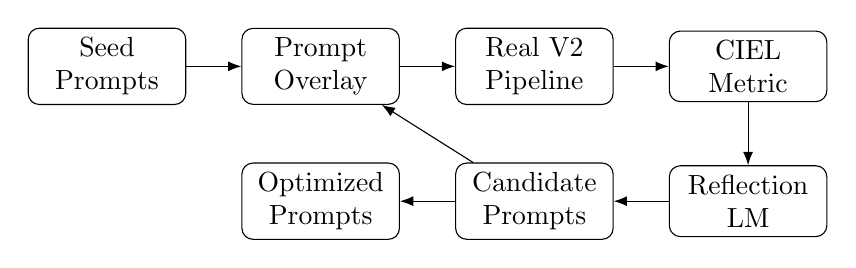
\begin{tikzpicture}[
  box/.style={draw, rounded corners, align=center, minimum height=0.75cm, minimum width=2.0cm},
  arrow/.style={-Latex},
  node distance=0.8cm and 0.7cm
]
\node[box] (seed) {Seed\\Prompts};
\node[box, right=of seed] (overlay) {Prompt\\Overlay};
\node[box, right=of overlay] (pipeline) {Real V2\\Pipeline};
\node[box, right=of pipeline] (metric) {CIEL\\Metric};
\node[box, below=of metric] (reflect) {Reflection\\LM};
\node[box, left=of reflect] (candidate) {Candidate\\Prompts};
\node[box, left=of candidate] (export) {Optimized\\Prompts};
\draw[arrow] (seed) -- (overlay);
\draw[arrow] (overlay) -- (pipeline);
\draw[arrow] (pipeline) -- (metric);
\draw[arrow] (metric) -- (reflect);
\draw[arrow] (reflect) -- (candidate);
\draw[arrow] (candidate) -- (overlay);
\draw[arrow] (candidate) -- (export);
\end{tikzpicture}
\caption{GEPA optimization loop for production prompts.}
\end{figure}

The GEPA score is normalized to a 0 to 1 range. A score of 1.0 means full CIEL-expanded cluster coverage with a valid schema and acceptable field count. The reported 0.246 form score comes from a small CIEL-focused optimization subset where the goal was to improve concept selection behavior under difficult terminology conditions. The broader 147-prompt form-builder baseline is reported separately as the system-level form evaluation. Because this is a CIEL-focused calibration subset, the score is best read as evidence for the optimization loop under difficult terminology conditions rather than as a broad product-quality score.

Internal technical evaluation metrics:

\begin{itemize}
  \item Baseline form-builder eval: 147/147 completed prompts, 0 failures, mean recall 0.465, schema-valid rate 0.993, median latency 17.97 s.
  \item Historical form CIEL GEPA run: best validation score 0.246 on a small dev subset.
  \item Historical report GEPA run: best validation score 0.492 on a small report GEPA subset.
\end{itemize}

These are reported as completed internal technical evaluation results for the submitted system.

\section{LoRA Fine-Tuning}

TenaOS ships a single task-tagged LoRA adapter that serves every workflow. Rather than maintaining one model per feature, the adapter is trained multi-task over clinical-informatics behaviours and routed at inference by task tags such as \texttt{[form]}, \texttt{[report]}, \texttt{[scribe]}, \texttt{[scribe-am]}, \texttt{[cds]}, and \texttt{[edu]}.

The sibling LoRA repository generates, validates, normalizes, and trains the adapter corpus:

\begin{itemize}
  \item 16,005 validated task-tagged traces,
  \item 18,909 training conversations,
  \item 1,071 validation conversations,
  \item 1,109 held-out test conversations.
\end{itemize}

The form trace schema teaches assistant-side behavior: understanding requests, planning evidence search, searching \WHO{} evidence, selecting \CIEL{} concepts, building a final form, and marking quality. Validation rejects PHI-like samples, invalid schema states, retired concepts, wrong datatypes, duplicate CIEL codes, unsupported concepts, unresolved items, and records outside the training-readiness criteria.

The adapter was trained as a BF16 LoRA over the text decoder. Records are real multi-turn ShareGPT-style conversations reconstructed from production event traces where available, and training masks loss to assistant turns only. Training used rank 16, alpha 32, dropout 0.0, maximum sequence length 24,576, batch size 1 with 8-step gradient accumulation, and 3 epochs. Runtime was 70.5 hours on an A100 80GB, and the final recorded train loss was 0.04123. Workflow-level LoRA performance claims require a separate full-runtime evaluation.

\section{Evaluation Methodology}

The core principle is to separate technical evaluation from clinical validation.

\begin{longtable}{p{0.22\linewidth}p{0.43\linewidth}p{0.25\linewidth}}
\toprule
\textbf{Workflow} & \textbf{Key metrics} & \textbf{Completed evidence in this report} \\
\midrule
Form builder and GEPA & CIEL-expanded recall, exact recall, schema-valid rate, size-ok rate, hallucinated-code rate, retired-code rate, tool calls, latency, publish readiness & 147/147 form prompts completed, 0 failures, 0.465 mean concept-cluster recall, 0.993 schema-valid rate, 17.97 s median latency \\
\addlinespace
WHO/MSF retrieval & Retrieval scale, local indexing, hybrid retrieval, reranker design, citation grounding & 69,476 guideline chunks indexed with EmbedGemma dense vectors and BM25 sparse vectors; 448.8 MB local Qdrant snapshot \\
\addlinespace
CIEL retrieval and validation & Concept coverage, mapping coverage, retired concept handling, bundle hydration, OpenMRS concept identity & 58,687 concepts, 298,905 mappings, 8,545 Q-and-A edges, 3,259 concept-set edges, 58,687 hydrated bundles \\
\addlinespace
Scribe & Text and voice input path, SOAP extraction, CIEL concept resolution, unresolved-item handling, clinician confirmation & Text, voice, and Amharic trace corpus included in LoRA training; workflow extraction and WER evaluation remain separate \\
\addlinespace
Report builder & Report spec grammar, CIEL filter validation, datatype-specific FHIR plan compilation, deterministic execution boundary & Compiler implemented with Boolean, coded, numeric, condition, and any-value filter modes \\
\addlinespace
CDS and patient education & WHO/MSF retrieval, cited output generation, abstention posture, clinician review & Agentic guideline search and cited output workflows implemented over local WHO/MSF KB \\
\addlinespace
Deployment & Local artifact footprint, model serving, Qdrant restore, single-container operation & Single-container Docker Compose runtime implemented; artifact bootstrap documented in \texttt{scripts/fetch-models.sh}; Qdrant restore documented in \texttt{docker/restore-qdrant.sh}; measured release artifacts include Gemma 4 E4B BF16 GGUF plus mmproj, 448.8 MB guideline snapshot, and 326.3 MB CIEL snapshot \\
\bottomrule
\end{longtable}

\section{Responsible AI and Safety}

\Product{} is built around layered controls:

\begin{itemize}
  \item \textbf{Local data boundary:} \OpenMRS{}, model inference, \CIEL{}, Qdrant, and trace stores run locally.
  \item \textbf{Allow-listed tools:} Gemma uses exposed allow-listed tools.
  \item \textbf{Retrieval grounding:} CDS and patient education use retrieved \WHO{} evidence.
  \item \textbf{Terminology validation:} final clinical records use \CIEL{} bundles and \OpenMRS{} concept IDs.
  \item \textbf{Deterministic middleware:} schema builds, report plans, concept filters, and \OpenMRS{} writes are compiled and checked outside the model.
  \item \textbf{Human review:} forms, scribe outputs, patient materials, and clinical recommendations are reviewable before use.
  \item \textbf{Audit traces:} workflows persist or stream tool calls, retrieval results, and draft evolution.
\end{itemize}

\section{Clinical Governance Boundary}

\Product{} uses a clinical governance boundary: the system produces evidence-grounded, standards-based drafts that pass through deterministic validation and clinician review before clinical persistence. The completed evidence package in this report includes implementation evidence, local corpus and index measurements, deterministic validation design, and internal technical evaluation runs.

\section{Reproducibility}

Important entry points:

\begin{itemize}
  \item Runtime setup: \texttt{README.md}, \texttt{scripts/setup-demo.sh}, \texttt{scripts/fetch-models.sh}.
  \item Agent workflows: \texttt{TenaAgent/README.md}, \texttt{TenaAgent/service/tena\_agent\_service/}.
  \item \WHO{} KB runtime: \texttt{TenaOS-KnowledgeBase/}.
  \item \WHO{} KB build: \texttt{/var/www/TenaOS\_DeepSeek/kb-pipeline/}.
  \item \CIEL{} build/runtime: \texttt{TenaOS-CIEL/}.
  \item GEPA optimization: \texttt{scripts/optimization/}.
  \item Evaluation protocol: \texttt{docs/evaluation/evaluation-protocol.md}.
  \item Evidence ledger: \texttt{docs/evaluation/evidence-ledger.md}.
  \item Diagram source: \texttt{docs/technical-report-assets/architecture-diagrams.md}.
\end{itemize}

\section{References}

\begin{itemize}
  \item \OpenMRS{}: open-source medical record system.
  \item \CIEL{}: Columbia International eHealth Laboratory concept dictionary.
  \item FHIR R4: reporting read interface through \OpenMRS{} FHIR2.
  \item WHO and MSF clinical guidance: local guideline evidence corpus.
  \item \Gemma{}: local multimodal generation model.
  \item EmbedGemma 300M: dense retrieval model for guideline chunks.
  \item SapBERT: dense biomedical concept encoder for \CIEL{} semantic search.
  \item Qdrant: local vector database for dense and sparse retrieval.
  \item GEPA/DSPy: offline prompt optimization framework.
\end{itemize}

\end{document}
